\documentclass[11pt]{article}
\usepackage{amsmath, amssymb}
\usepackage[margin=1in, top=0.8in, bottom=0.8in]{geometry}
\usepackage{parskip}
\usepackage{xcolor}
\usepackage{mdframed}
\usepackage{titlesec}
\usepackage{fancyhdr}
\usepackage{enumitem}
\usepackage{graphicx}
\usepackage{hyperref}

\definecolor{headingblue}{RGB}{30, 70, 130}
\definecolor{boxbg}{RGB}{240, 245, 255}
\definecolor{boxborder}{RGB}{30, 70, 130}

% Section formatting
\titleformat{\section}{\large\bfseries\color{headingblue}}{}{0em}{}[\titlerule]
\titleformat{\subsection}{\normalsize\bfseries\color{headingblue}}{}{0em}{}
\titlespacing{\section}{0pt}{10pt}{5pt}
\titlespacing{\subsection}{0pt}{8pt}{3pt}

% Result box
\newmdenv[
  backgroundcolor=boxbg,
  linecolor=boxborder,
  linewidth=1.5pt,
  roundcorner=4pt,
  innertopmargin=8pt,
  innerbottommargin=8pt,
  innerleftmargin=12pt,
  innerrightmargin=12pt,
  skipabove=8pt,
  skipbelow=6pt,
]{resultbox}

% Header
\pagestyle{fancy}
\fancyhf{}
\rhead{\textcolor{headingblue}{\small SMAI S26}}
\lhead{\textcolor{headingblue}{\small Conjugate Priors}}
\cfoot{\thepage}
\renewcommand{\headrulewidth}{0.4pt}

\hypersetup{
  colorlinks=true,
  linkcolor=headingblue,
  urlcolor=headingblue,
  citecolor=headingblue
}

\setlength{\parskip}{5pt}

\begin{document}

% Title block
\begin{center}
  {\LARGE\bfseries\color{headingblue} CONJUGATE PRIORS}\\[0.5em]
  {\large Krishna Jakka \quad \texttt{2023101058}}
\end{center}

\vspace{0.5em}

% -------------------------------------------------------
\section{Intuition}

\subsection{Parametric Families}

A parametric family is a collection of probability distributions that are all described by the same general form, but differ based on the value of one or more parameters. For example, all normal distributions, regardless of their specific mean or variance, belong to the same parametric family, since they share the same underlying shape and are fully characterized by just those two values.

\subsection{Conjugate Priors}

In Bayesian inference, we start with a \textbf{prior distribution} which reflects our initial beliefs about the unknown parameter before we observe any data. Once we observe data, we use the prior distribution and the likelihood of observing the data to compute a \textbf{posterior distribution}, which is an updated version of our beliefs. Note that the process is sequential in nature; i.e., the posterior distribution obtained in the previous step is used as the prior distribution in the next step.

A \textbf{conjugate prior} is a prior distribution such that when it is used with a certain type of likelihood distribution, it results in a posterior distribution of the same type as the prior distribution. That is, the type of distribution we use in Bayesian inference remains the same throughout the process; only the parameters of the distribution change. This is an important property of conjugate priors because it ensures that we never encounter an intractable form while sequentially updating our beliefs using observed data.

% -------------------------------------------------------
\section{Worked Example}

To solidify the concept discussed so far, it is useful to look at a worked example. It can easily be proved that a Gaussian prior with Gaussian likelihood yields a Gaussian posterior, which is done below.

\subsection*{Setup}

Let $x_1, \ldots, x_n \mid \mu \sim \mathcal{N}(\mu, \sigma^2)$ with $\sigma^2$ known, and place a Gaussian prior $\mu \sim \mathcal{N}(\mu_0, \tau^2)$. We derive the posterior $p(\mu \mid \mathbf{x})$ via Bayes' theorem:
\[
  p(\mu \mid \mathbf{x}) \;\propto\; p(\mathbf{x} \mid \mu)\,p(\mu)
\]

\subsection*{Combining Likelihood and Prior}

Working with log-kernels and dropping constants in $\mu$, the log-likelihood contributes $-\frac{1}{2\sigma^2}\sum_i(x_i - \mu)^2$, which expands to $-\frac{1}{2\sigma^2}(n\mu^2 - 2n\bar{x}\mu)$, and the log-prior contributes $-\frac{1}{2\tau^2}(\mu^2 - 2\mu_0\mu)$. Adding these:
\[
  \log p(\mu \mid \mathbf{x}) \;\propto\; -\frac{1}{2}\left[
    \underbrace{\left(\frac{n}{\sigma^2} + \frac{1}{\tau^2}\right)}_{a}\mu^2
    - 2\underbrace{\left(\frac{n\bar{x}}{\sigma^2} + \frac{\mu_0}{\tau^2}\right)}_{b}\mu
  \right]
\]

\subsection*{Completing the Square}

Using $a\mu^2 - 2b\mu = a(\mu - b/a)^2 - b^2/a$ and absorbing the constant term:
\[
  p(\mu \mid \mathbf{x}) \;\propto\; \exp\!\left(-\frac{a}{2}\!\left(\mu - \frac{b}{a}\right)^{\!2}\right)
\]

This is the kernel of a Gaussian with mean $\mu_n = b/a$ and variance $\tau_n^2 = 1/a$.

\subsection*{Posterior Parameters}

\begin{resultbox}
\textbf{Posterior:} $\quad\mu \mid \mathbf{x} \;\sim\; \mathcal{N}(\mu_n,\,\tau_n^2)$
\vspace{0.5em}
\[
  \tau_n^2 = \frac{1}{\dfrac{n}{\sigma^2} + \dfrac{1}{\tau^2}}, \qquad
  \mu_n = \tau_n^2\!\left(\frac{n\bar{x}}{\sigma^2} + \frac{\mu_0}{\tau^2}\right)
\]
\end{resultbox}

The posterior mean can be expressed as a \textbf{precision-weighted average} of the prior mean and the sample mean. Defining prior precision $\lambda = 1/\tau^2$ and likelihood precision $\lambda_\ell = n/\sigma^2$:
\[
  \mu_n \;=\; \frac{\lambda\,\mu_0 + \lambda_\ell\,\bar{x}}{\lambda + \lambda_\ell}
\]

This confirms that the Gaussian prior is conjugate to the Gaussian likelihood: the posterior is Gaussian, belonging to the same parametric family as the prior, with parameters updated cleanly in closed form. $\blacksquare$

\subsection*{Visual Illustration}

Figure~\ref{fig:gaussian_conjugate} illustrates the above derivation with a concrete numerical example. The prior (blue) is broad and centered near zero, reflecting substantial uncertainty about $\mu$ before any data is observed. The likelihood (orange), treated as a function of $\mu$, is narrow and shifted to the right, reflecting strong information from the data. The posterior (green) combines both sources — it is narrower than the prior (reduced uncertainty) and pulled toward the likelihood (data has updated our beliefs). Crucially, all three curves are Gaussian, visually confirming the conjugacy property.

% ---- GAUSSIAN CONJUGATE PRIOR SIMULATION ----
\vspace{0.3em}
\begin{center}
\begin{tabular}{lccc}
  \hline
  \textbf{Distribution} & \textbf{Mean} & \textbf{Variance} & \textbf{Notes} \\
  \hline
  Prior $p(\mu)$                    & $\mu_0 = 0.50$ & $\tau^2 = 1.0000$       & Prior belief \\
  Likelihood $p(\mathbf{x}\mid\mu)$ & $\bar{x} = 2.906$ & $\sigma^2/n = 0.0613$ & $n = 8$ observations \\
  Posterior $p(\mu\mid\mathbf{x})$  & $\mu_n = 2.768$ & $\tau_n^2 = 0.0577$     & Precision-weighted update \\
  \hline
\end{tabular}
\end{center}
\vspace{0.3em}

\begin{figure}[h]
  \centering
  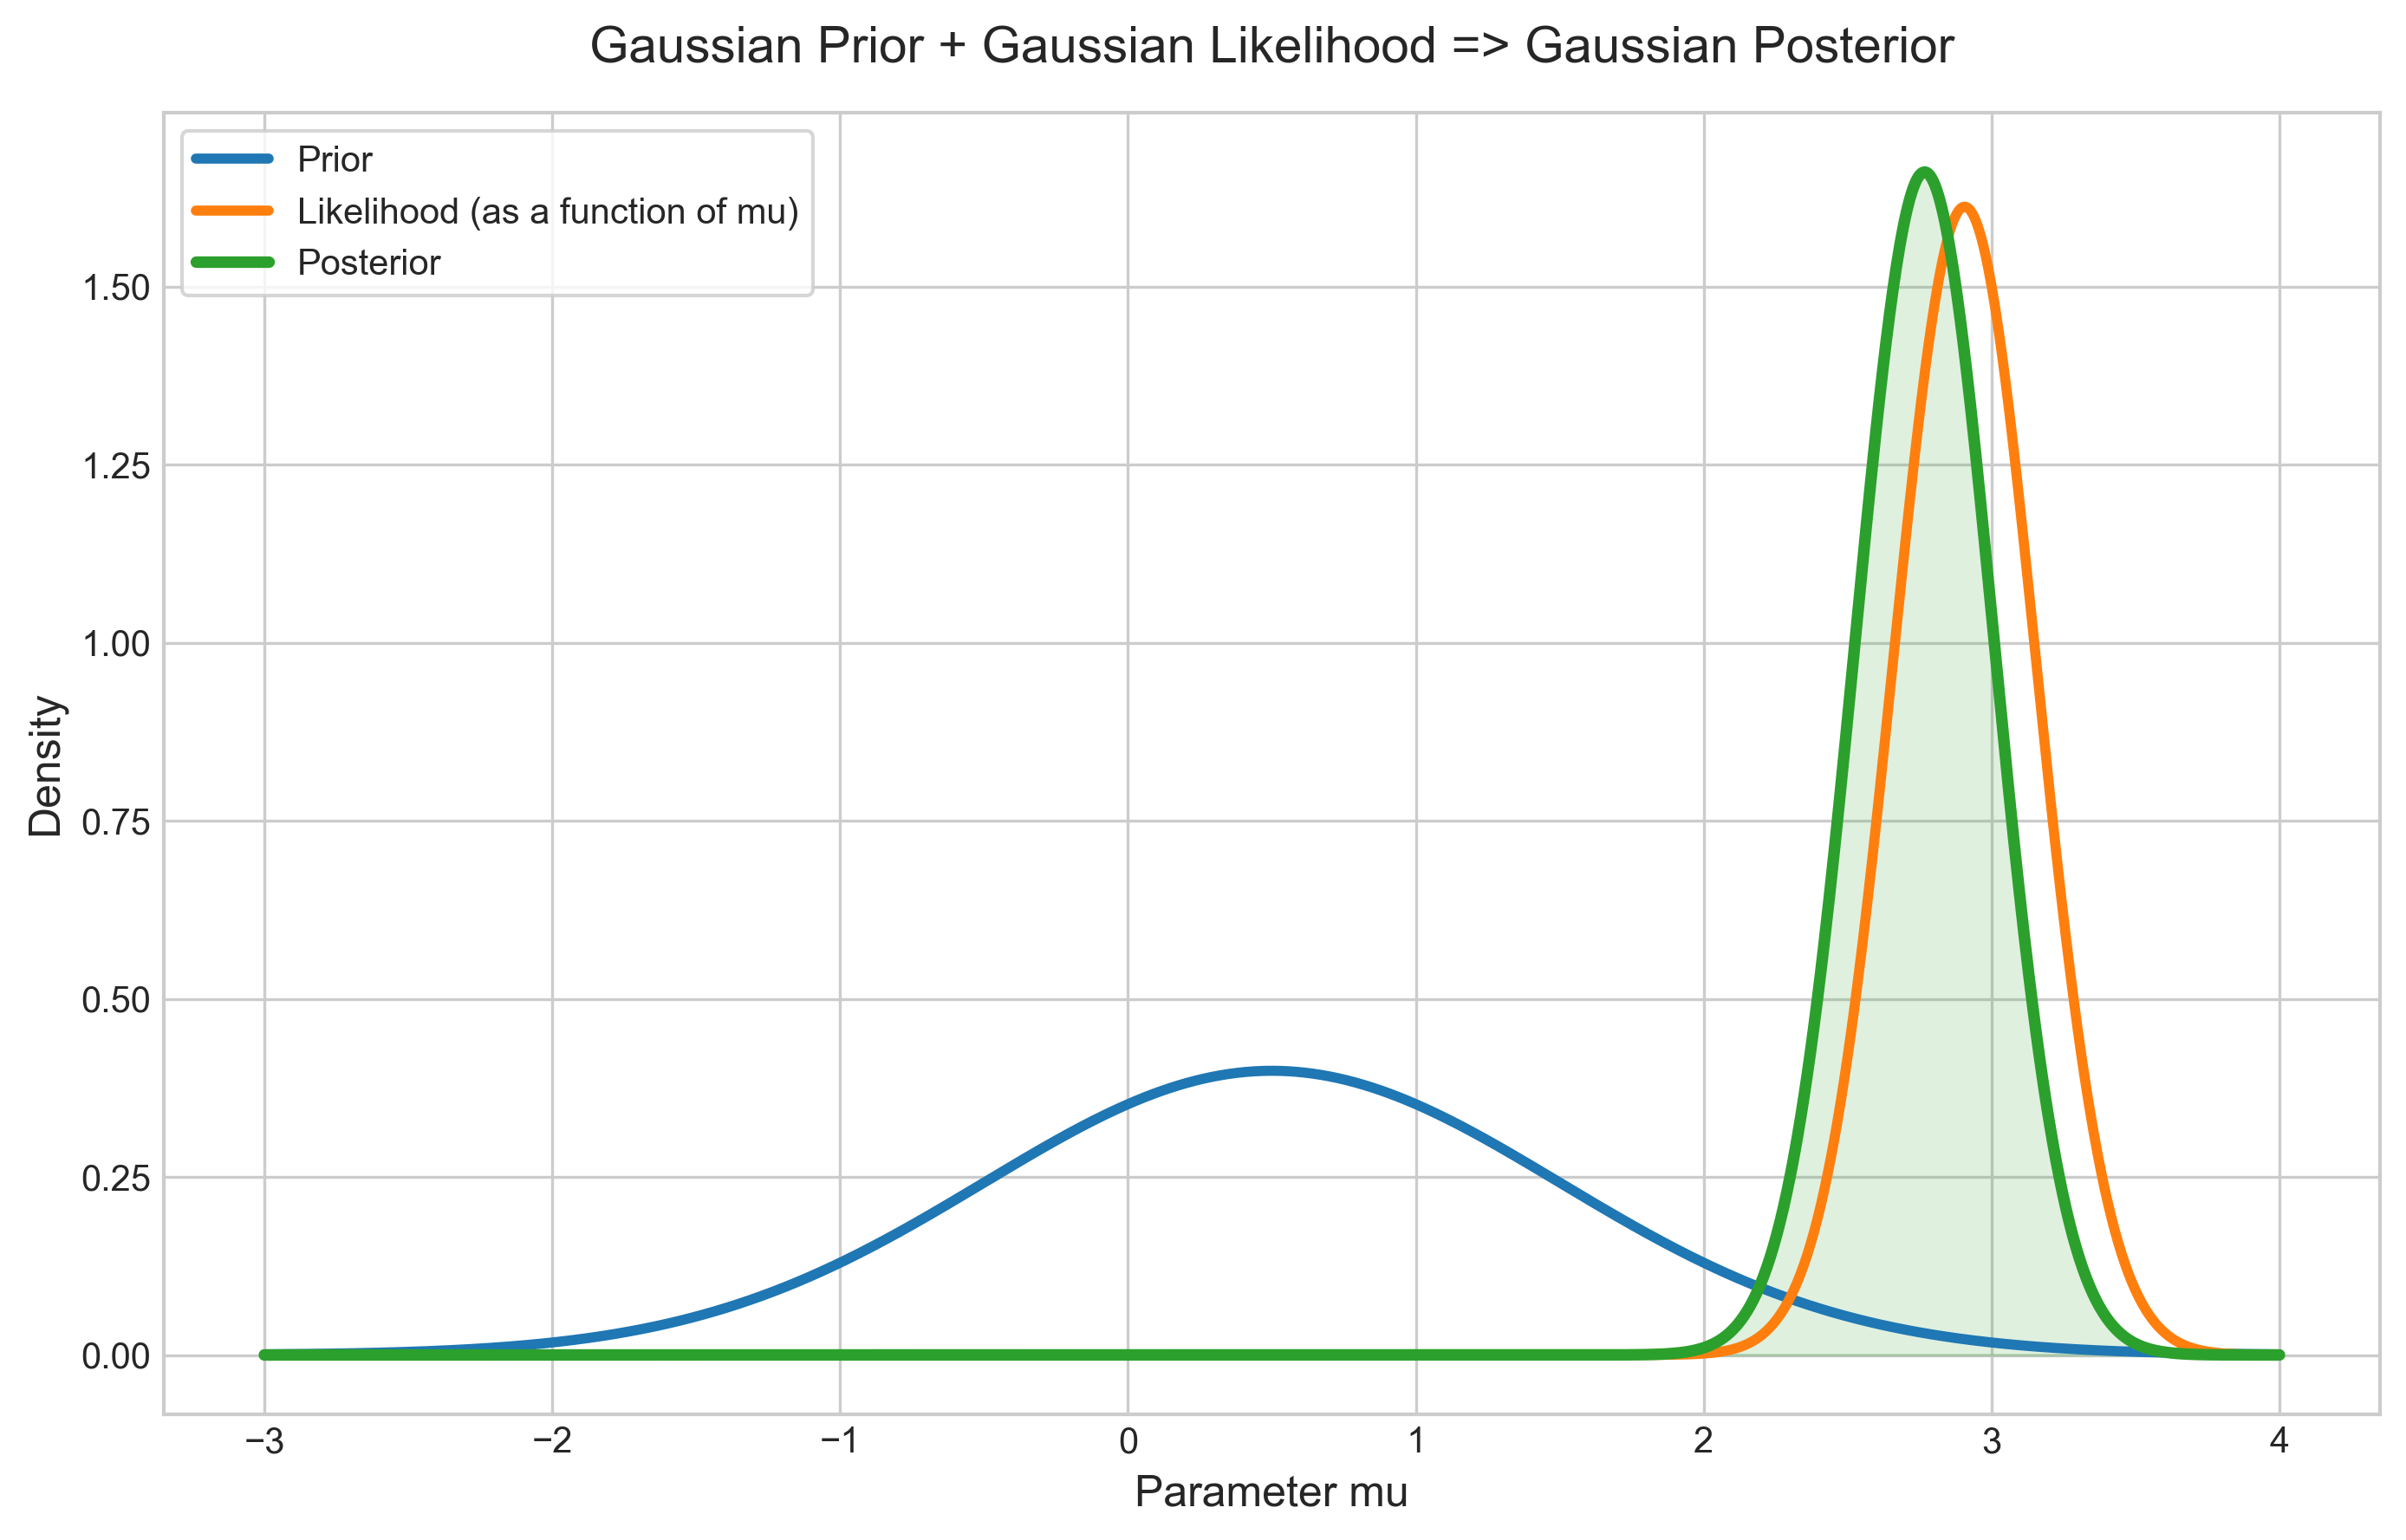
\includegraphics[width=0.85\textwidth]{conjugate_priors_plot.png}
  \caption{Gaussian prior, likelihood (as a function of $\mu$), and the resulting Gaussian posterior. The posterior is narrower than the prior and its mean lies between the prior mean and the sample mean, pulled proportionally by each distribution's precision.}
  \label{fig:gaussian_conjugate}
\end{figure}

% -------------------------------------------------------
\section{Application in Bayesian Updating}

The practical power of conjugate priors becomes most evident when we apply Bayesian inference repeatedly. This happens naturally when data comes in batches or streams over time. In any Bayesian framework, the posterior from one round of inference serves as the prior for the next. The question is what form that posterior takes after each update.

Without conjugacy, the posterior can become a complicated distribution after even a single update. It might not have a closed-form expression and could require numerical approximation. This issue worsens with each sequential step: every update could create a more complex posterior, making the calculations more costly.

Conjugate priors completely solve this problem. Since the posterior always stays within the same parametric family as the prior, we can summarize our beliefs at any time with a fixed, limited set of parameters. Updating those beliefs when new data arrives becomes a simple parameter update; no need to re-derive or use numerical approximation. In the Gaussian case discussed earlier, this means that no matter how many updates have happened, beliefs about $\mu$ are always expressed as $\mathcal{N}(\mu_n, \tau_n^2)$. The values of $\mu_n$ and $\tau_n^2$ change with each new data batch based on the earlier derived closed-form expressions.

This also provides clear interpretability. The hyperparameters of a conjugate prior often have direct meaning. In the Gaussian case, $\mu_0$ represents our best guess for $\mu$ before we see any data, and $\tau^2$ shows how confident we are in that guess. After observing data, $\mu_n$ and $\tau_n^2$ update in a way that is easy to understand as a balance between prior belief and new evidence. This clarity makes conjugate models not only easy to compute but also genuinely informative about how and why our beliefs change.

% -------------------------------------------------------
\section{References}

\begin{enumerate}[leftmargin=*, label={[\arabic*]}]

  \item \textit{What is a conjugate prior?}\\
  Ben Lambert, YouTube \\
  \url{https://www.youtube.com/watch?v=aPNrhR0dFi8}

  \item \textit{
Bayesian Updating | Probability and statistics}\\
  Math and Adventures, YouTube\\
  \url{https://www.youtube.com/watch?v=p0ybAJMHNtE}

  \item \textit{
Bayesian Updates and Conjugate Priors}\\
  Steve Brunton, YouTube\\
  \url{https://www.youtube.com/watch?v=GqSX-8AQL90}

  \item \textit{
Bayesian Updating Simply Explained}\\
  Egor Howell\\
  \url{https://towardsdatascience.com/bayesian-updating-simply-explained-c2ed3e563588/}

  \item Taboga, Marco (2021). "Conjugate prior", Lectures on probability theory and mathematical statistics. Kindle Direct Publishing. Online appendix.\\
  \url{https://www.statlect.com/fundamentals-of-statistics/conjugate-prior}

  \item Code used for generating the plot:\\
  \url{https://github.com/KJsquare9/smai_a1_q4.git}

\end{enumerate}

\end{document}
